\documentclass{llncs}
\usepackage{amsmath,amssymb}
\usepackage{makeidx}  % allows for indexgeneration
%

\usepackage[american]{babel}
\usepackage[utf8]{inputenc}

\usepackage{float}
\let\proof\relax
\let\endproof\relax
\usepackage{amsthm}
\usepackage{color}
\usepackage{fancyhdr}
\usepackage{hyperref}
\usepackage{graphicx}
\usepackage{float}
%\usepackage{minted}

\newcommand{\idris}[1]{\texttt{#1}}%{\mintinline{idris}{#1}}
\newcommand{\haskell}[1]{\texttt{#1}}%{\mintinline{haskell}{#1}}
\newtheorem{Lemma}{Lemma}
\newtheorem{Theorem}{Theorem}
\begin{document}


%
\mainmatter              % start of the contributions

\title{Certified Derivative-Based Parsing of Regular Expressions}

%
\author{Raul Lopes\inst{1} \and Rodrigo Ribeiro \inst{2} \and Carlos Camar\~ao\inst{3}}
\institute{DECOM, Universidade Federal de Ouro Preto (UFOP), Ouro Preto\\
\email{raulfpl@gmail.com} \and
DECSI, Universidade Federal de Ouro Preto (UFOP), João Monlevade\\
\email{rodrigo@decsi.ufop.br} \and
DCC, Universidade Federal de Minas Gerais (UFMG), Belo Horizonte\\
\email{camarao@dcc.ufmg.br}
}
\maketitle              % typeset the title of the contribution

\begin{abstract}
We describe the formalization of a certified algorithm for regular
expression parsing based on Brzozowski derivatives, in the dependently
typed language Idris. The formalized algorithm produces a proof that
an input string matches a given regular expression or a proof that no
matching exists. A tool for regular expression based search in the
style of the well known GNU grep has been developed with the certified
algorithm, and practical experiments were conducted with this tool.
\end{abstract}


\section{Introduction}\label{sec:intro}

Parsing is the process of analysing if a string of symbols conforms to
given rules, involving also, in computer science, formally specifying
the rules in a grammar and also, either the construction of data that
makes evident the rules that have been used to conclude that the
string of symbols can be obtained from the grammar rules, or else
indication of an error, representative of the fact that the string of
symbols cannot be generated from the grammar rules.

In this work, we are interested in the parsing problem for regular
languages (RLs)~\cite{Hopcroft2000}, i.e. languages recognized by
(non-)deterministic finite automata and equivalent formalisms. Regular
expressions (REs) are an algebraic and compact way of specifying RLs
that are extensively used in lexical analyser
generators~\cite{Lesk1990} and string search utilities~\cite{Grep}.
Since such tools are widely used and parsing is pervasive in
computing, there is a growing interest on correct parsing
algorithms~\cite{FirsovU13,FirsovU14,Danielsson2010}.  This interest
is motivated by the recent development of dependently typed
languages. Such languages are powerful enough to express algorithmic
properties as types, that are automatically checked by a compiler.

The use of derivatives for regular expressions were introduced by
Brzozowski~\cite{Brzozowski1964} as an alternative method to compute a
finite state machine that is equivalent to a given RE and to perform
RE-based parsing. According to Owens et. al~\cite{Owens2009},
``derivatives have been lost in the sands of time'' until his work on
functional encoding of RE derivatives have renewed interest on its use
for parsing~\cite{Might2011,Fischer2010}.  In this work, we provide a
complete formalization of an algorithm for RE parsing using
derivatives, as presented by~\cite{Owens2009}, and describe a RE based
search tool that has been developed by us, using the dependently typed
language Idris.

More specifically, our contributions are:
\begin{itemize}
  \item A formalization of derivative based regular expression parsing
    in Idris. The certified RE parsing algorithm presented produces as
    a result either a proof term (parse tree) that is evidence that
    the input string is in the language of the input RE, or a witness
    that such parse tree does not exist.

  \item A detailed explanation of the technique used to quotient
    derivatives with respect to ACUI axioms\footnote{Associativity,
      Commutativity and Idempotence with Unit elements axioms for
      REs~\cite{Brzozowski1964}.} in an implementation by Owens et
    al.~\cite{Owens2009}, called ``smart-constructors'', and its proof
    of correctness. We give formal proofs that smart constructors
    indeed preserve the language recognized by REs.
\end{itemize}

The rest of this paper is organized as
follows. Section~\ref{sec:idris} presents a brief introduction to
Idris. Section~\ref{sec:regexp} describes the encoding of REs and its
parse trees. In Section~\ref{sec:deriv} we define derivatives and
smart constructors, some of their properties and describe how to build
a correct parsing algorithm from them. Section~\ref{sec:exp} comments
on the usage of the certified algorithm to build a tool for RE-based
search and present some experiments with it. Related work is discussed
on Section~\ref{sec:related}.  Section~\ref{sec:conclusion} concludes.

All the source code in this article has been formalized in Idris
version 0.11, but
we do no present every detail. Proofs of some properties result in
functions with a long pattern matching structure, that would distract
the reader from understanding the high-level structure of the
formalization. In such situations we give just proof sketchs and point
out where all details can be found in the source code.

The complete Idris development, instructions on how to build and use
it can be found at~\cite{regex-rep}.

\section{An Overview of Idris}\label{sec:idris}

Idris~\cite{Brady2013} is a dependently typed functional programming
language that focus on supporting practical programs. Idris syntax is
inspired by Haskell’s with some minor differences. Unlike Haskell,
Idris is strict by default, but lazy evaluation is supported through
code annotations. Idris allows the definition of datatypes using
traditional Haskell and a GADT-style syntax.  The type of types is
called \idris{Type}, rather than $\star$\footnote{In Haskell, types
  are classified using kinds~\cite{Pierce2002} instead of universe
  levels. The kind of types is denoted by $\star$ and type operators
  have functional kinds: $\kappa\to\kappa'$, where $\kappa$ and
  $\kappa'$ are kinds. As an example, in Haskell, type \haskell{Bool}
  has kind $\star$ and the list type constructor has kind
  $\star\to\star$.}. Each instance of \idris{Type} has an implicit
level, inferred by the compiler. Levels are cumulative --- everything
in \idris{Type}$_n$ is also in \idris{Type}$_{n+1}$.

As an example of Idris code, consider the following data type of
length-indexed lists, also known as vectors.
\begin{verbatim}
data Nat = Z | S Nat
data Vec : Nat -> Type -> Type where
    Nil : Vec Z a
    (::) : a -> Vec n a -> Vec (S n) a
\end{verbatim}
Constructor \idris{Nil} builds empty vectors. The cons-operator
inserts a new element in front of a vector of $n$ elements (of type
\idris{Vec n a}) and returns a value of type \idris{Vec (S n) a}. The
\idris{Vec} datatype is an example of a dependent type, i.e. a type
that uses a value (that denotes its length). The usefulness of
dependent types can be illustrated with the definition of a safe list
head function: \idris{head} can be defined to accept only non-empty
vectors, i.e.~values of type \idris{Vec (S n) a}.
\begin{verbatim}
head : Vec (S n) a -> a
head (x :: xs) = x
\end{verbatim}
In \idris{head}'s definition, constructor \idris{Nil} is not used. The
Idris type-checker can figure out, from \idris{head}'s parameter type,
that argument \idris{Nil} to \idris{head} is not type-correct.

In Idris, free variables that start with a lower-case letter are
considered to be implicit arguments, i.e.~arguments that can be
automatically infered by the compiler. It is also possible to mark
arguments as implicit by surrounding them in curly braces. In function
\idris{head}, both \idris{n : Nat} and \idris{a : Type} are implicit
arguments; they could be explicitly annotated in \idris{head}'s type
as follows:
\begin{verbatim}
head : {a : Type} -> {n : Nat} -> Vec (S n) a -> a
\end{verbatim}

Thanks to the propositions-as-types principle\footnote{Also known as
  Curry-Howard ``isomorphism''~\cite{Sorensen2006}.} we can interpret
types as logical formulas and terms as proofs. An example is the
representation of equality as the following Idris type:
\begin{verbatim}
data (=) : a -> b -> Type where
   Refl : x = x
\end{verbatim}
This type is called propositional equality\footnote{Readers who know
  type theory probably have noticed that this equality encoding
  corresponds to the so-called heterogeneous
  equality~\cite{McBride1999}, which is used in the Idris
  Prelude. Detailed discussions about equality in type theory can be
  found in~\cite{Hott}.}. It defines that there is a unique evidence
for equality, constructor \idris{Refl} (for reflexivity), that asserts
that the only value equal to $x$ is itself. Given a type \idris{P},
type \idris{Dec P} is used to build proofs that \idris{P} is a
decidable proposition, i.e.~that either \idris{P} or not \idris{P}
holds. The decidable proposition type is defined as:
\begin{verbatim}
data Dec : Type -> Type where
     Yes : p -> Dec p
     No : Not p -> Dec p
\end{verbatim}
Constructor \idris{Yes} stores a proof that property \idris{P} holds
and \idris{No} an evidence that such proof is impossible (\idris{Not}
is an implication of falsity). Some functions used in our
formalization use this type.

Dependently typed pattern matching is built by using the so-called
\idris{with} construct, that allows for matching intermediate
values~\cite{McBride2004}. If the matched value has a dependent type,
then its result can affect the form of other values. For example,
consider the following code that defines a type for natural number
parity. If the natural number is even, it can be represented as the
sum of two equal natural numbers; if it is odd, it is equal to one
plus the sum of two equal values. Pattern matching on a value of
\idris{Parity n} allows to discover if $n = j + j$ or $n = S (k + k)$,
for some $j$ and $k$ in each branch of \idris{with}.  Note that the
value of $n$ is specialized accordingly, using information ``learned''
by the type-checker.
\begin{verbatim}
data Parity : Nat -> Type where
   Even : Parity (n + n)
   Odd  : Parity (S (n + n))

parity : (n : Nat) -> Parity n
parity = -- definition omitted

natToBin : Nat -> List Bool
natToBin Z = Nil
natToBin k with (parity k)
   natToBin (j + j)     | Even = False :: natToBin j
   natToBin (S (j + j)) | Odd  = True  :: natToBin j
\end{verbatim}

A detailed discussion about the Idris language is out of the scope of
this paper. A tutorial on Idris is available \cite{idris-tutorial}.

\section{Regular Expressions}\label{sec:regexp}

Regular expressions are defined with respect to a given
alphabet. Formally, RE syntax follows the following context-free
grammar
\[
e ::= \emptyset\,\mid\,\epsilon\,\mid\,a\,\mid\,e\,e\,\mid\,e+e\,\mid\,e^{\star}
\]
where $a$ is a symbol from the underlying alphabet.  In our
formalization, we describe symbols of an alphabet as a natural number
in Peano notation (type \idris{Nat}), i.e.~the symbol's numeric
code. The reason for this design choice is due to the way that Idris
deals with propositional equality for primitive types, like
\idris{Char}. Equalities of values of these types only reduce on
concrete primitive values; this causes computation of proofs to stop
under variables whose type is a primitive one. Thus, we decide to use
the inductive type \idris{Nat} to represent the codes of alphabet
symbols, since computation of its equality proofs behaves as expected
in other languages, like e.g.~Agda~\cite{Norell2009}.
% Nao entendi o que esta sendo falado neste paragrafo:
% why Chr nao tem o tipo Char -> RegExp ?


Datatype \idris{RegExp}, defined below, encodes RE syntax:
\begin{verbatim}
data RegExp : Type where
  Zero : RegExp
  Eps  : RegExp
  Chr  : Nat -> RegExp
  Cat  : RegExp -> RegExp -> RegExp
  Alt  : RegExp -> RegExp -> RegExp
  Star : RegExp -> RegExp
\end{verbatim}
Constructors \idris{Zero} and \idris{Eps} denote respectively the
empty language ($\emptyset$) and empty string ($\epsilon$). Alphabet
symbols are constructed using \idris{Chr} constructor. Bigger REs are
built using concatenation (\idris{Cat}), union (\idris{Alt}) and
Kleene star (\idris{Star}).
% nao seria melhor choice, em vez de union?

Using the datatype for RE syntax, we can define a relation for RL
membership. Such relation can be understood as a parse tree (or a
proof term) that a string, represented by a list of \idris{Nat}
values, belongs to the language of a given
RE. Datatype \idris{InRegExp} defines RE semantics inductively.

\begin{verbatim}
data InRegExp : List Nat -> RegExp -> Type where
  InEps : InRegExp [] Eps
  InChr : InRegExp [ a ] (Chr a)
  InCat : InRegExp xs l ->
          InRegExp ys r ->
          zs = xs ++ ys ->
          InRegExp zs (Cat l r)
  InAltL : InRegExp xs l ->
           InRegExp xs (Alt l r)
  InAltR : InRegExp xs r ->
           InRegExp xs (Alt l r)
  InStar : InRegExp xs (Alt Eps (Cat e (Star e))) ->
           InRegExp xs (Star e)
\end{verbatim}

Each constructor of \idris{InRegExp} datatype specifies how to build a
parse tree for some string and RE. Constructor \idris{InEps} states
that the empty string (denoted by the empty list \idris{[]}) is in the
language of RE \idris{Eps}. Parse tree for single characters are built
with \idris{InChr a}, which says that the singleton string
\idris{[ a ]} is in RL for \idris{Chr a}. Given parse trees for REs
\idris{l} and \idris{r}; \idris{InRegExp xs l} and \idris{InRegExp ys
  r}, we can use constructor \idris{InCat} to build a parse tree for the
concatenation of these ERs. Constructor \idris{InAltL}
(\idris{InAltR}) creates a parse tree for \idris{Alt l r} from a parse
tree from \idris{l}(\idris{r}). Parse trees for Kleene star are built
using the following well known equivalence of REs: $e^\star = \epsilon
+ e\,e^\star$.

Several inversion lemmas about RE parsing relation are necessary to
formalize derivative based parsing. They consist of pattern-matching
on proofs of \idris{InRegExp} and are omitted for brevity.
% nao seria bom incluir pelo menos um?

\section{Derivatives, Smart Constructors and Parsing}\label{sec:deriv}

\subsection{Preliminaries}

Formally, the derivative of a formal language $L\subseteq
\Sigma^\star$ with respect to a symbol $a\in\Sigma$ is the language
formed by suffixes of $L$ words without the prefix $a$.

An algorithm for computing the derivative of a language represented as
a RE as another RE is due to Brzozowski~\cite{Brzozowski1964} and it
relies on a function (called $\nu$) that determines if some RE accepts
or not the empty string:
% Following Owens et. al.~\cite{Owens2009}, this function is called $\nu$:
\[
    \begin{array}{lcl}
         \nu(\emptyset) & = & \emptyset \\
         \nu(\epsilon)    & = & \epsilon \\
         \nu(a)                & = & \emptyset \\
         \nu(e\,e')           & = & \left\{
                                                 \begin{array}{ll}
                                                      \epsilon &
                                                                 \text{if
                                                                 }\nu(e)
                                                                 =
                                                                 \nu(e')
                                                                 =
                                                                 \epsilon
                                                   \\
                                                   \emptyset &
                                                               \text{otherwise}
                                                 \end{array}
                                             \right. \\
         \nu(e + e')  & = & \left\{
                                         \begin{array}{ll}
                                              \epsilon & \text{if
                                                         }\nu(e) =
                                                         \epsilon
                                                         \text{ or
                                                         }\nu(e') =
                                                         \epsilon \\
                                              \emptyset & \text{otherwise}
                                         \end{array}
                                      \right. \\
         \nu(e^\star) & = & \epsilon
    \end{array}
\]
Decidability of $\nu(e)$ is proved by function \idris{hasEmptyDec},
which is defined by induction over the structure of the input RE
\idris{e} and returns a proof that the empty string is accepted or
not, using Idris type of decidable propositions, \idris{Dec P}.
\begin{verbatim}
hasEmptyDec : (e : RegExp) -> Dec (InRegExp [] e)
hasEmptyDec Zero = No (void . inZeroInv)
hasEmptyDec Eps = Yes InEps
hasEmptyDec (Chr c) = No inChrNil
hasEmptyDec (Cat e e') with (hasEmptyDec e)
  hasEmptyDec (Cat e e') | (Yes prf) with (hasEmptyDec e')
    hasEmptyDec (Cat e e') | (Yes prf) | (Yes prf')
          = Yes (InCat prf prf' Refl)
    hasEmptyDec (Cat e e') | (Yes prf) | (No contra)
          = No (contra . snd . inCatNil)
  hasEmptyDec (Cat e e') | (No contra)
          = No (contra . fst . inCatNil)
hasEmptyDec (Alt e e') with (hasEmptyDec e)
  hasEmptyDec (Alt e e') | (Yes prf)
          = Yes (InAltL prf)
  hasEmptyDec (Alt e e') | (No contra) with (hasEmptyDec e')
    hasEmptyDec (Alt e e') | (No contra) | (Yes prf)
          = Yes (InAltR prf)
    hasEmptyDec (Alt e e') | (No contra) | (No f)
          = No (void . either contra f . inAltNil)
hasEmptyDec (Star e)
          = Yes (InStar (InAltL InEps))
\end{verbatim}

\subsection{Smart Constructors}\label{sec:smart}

Following Owens et. al.~\cite{Owens2009}, we use smart constructors to
identify equivalent REs modulo identity and nullable
elements, $\epsilon$ and $\emptyset$, respectively. RE equivalence is
denoted by $e \approx e'$ and it's defined as usual~\cite{Hopcroft2000}.  The equivalence
axioms maintained by smart constructors are:
\begin{itemize}
    \item For union:
      \[
          \begin{array}{ccc}
              1)\: e + \emptyset \approx e &\hspace{1cm} & 2)\: \emptyset + e \approx e
          \end{array}
      \]
      \item For concatenation:
      \[
          \begin{array}{ccc}
              1)\: e\:\emptyset \approx \emptyset & \hspace{1cm} & 2)\: e\:\epsilon \approx e\\
              3)\: \emptyset\:e\approx \emptyset & & 4)\: \epsilon\: e \approx e\\
          \end{array}
      \]
      \item For Kleene star:
      \[
           \begin{array}{ccc}
               1)\: \emptyset^\star \approx \epsilon & \hspace{1cm} & 2)\: \epsilon^\star
                                                  \approx \epsilon
           \end{array}
      \]
\end{itemize}
These axioms are kept as invariants using functions that preserve them
while building REs. For union, we just need to worry when one
parameter denotes the empty language RE (\idris{Zero}):
\begin{verbatim}
(.|.) : RegExp -> RegExp -> RegExp
Zero .|. e = e
e .|. Zero = e
e .|. e'   = Alt e e'
\end{verbatim}
%seria bom deixar todos os .|. na mesma coluna.
In concatenation, we need to deal with the possibility of
parameters being the empty RE or the empty string RE. If one is the
empty language (\idris{Zero}) the result is also the empty
language. Since empty string RE is identity for concatenation, we
return, as a result, the other parameter.
\begin{verbatim}
(.@.) : RegExp -> RegExp -> RegExp
Zero .@. e = Zero
Eps .@. e  = e
e .@. Zero = Zero
e .@. Eps  = e
e .@. e'   = Cat e e'
\end{verbatim}
%seria bom deixar todos os .@. na mesma coluna.
For Kleene star both \idris{Zero} and \idris{Eps} are replaced by \idris{Eps}.
\begin{verbatim}
star : RegExp -> RegExp
star Zero = Eps
star Eps = Eps
star e = Star e
\end{verbatim}
Since all smart constructors produce equivalent REs, they preserve the
parsing relation. This property is stated as a soundness and
completeness lemma, stated below, of each smart constructor with
respect to \idris{InRegExp} proofs.
\begin{Lemma}[Soundness of union]
For all REs \idris{e}, \idris{e'} and all strings \idris{xs}, if
\idris{InRegExp xs (e .|. e')} holds then \idris{InRegExp xs (Alt e
  e')} also holds.
\end{Lemma}
\begin{proof}
  By case analysis on the structure of \idris{e} and \idris{e'}. The
  only interesting cases are when one of the expressions is
  \idris{Zero}. If \idris{e = Zero}, then \idris{Zero .|. e' = e'} and
  the desired result follows. The same reasoning applies for \idris{e'
  = Zero}.
\end{proof}
\begin{Lemma}[Completeness of union]
For all REs \idris{e}, \idris{e'} and all strings \idris{xs}, if
\idris{InRegExp xs (Alt e e')} holds then \idris{InRegExp xs (e
  .|. e')} also holds.
\end{Lemma}
\begin{proof}
   By case analysis on the structure of \idris{e}, \idris{e'}. The
   only interesting cases are when one of the REs is \idris{Zero}.  If
   \idris{e = Zero}, we need to analyse the structure of
   \idris{InRegExp xs (Alt e e')}. The result follows directly or by
   contradiction using \idris{InRegExp xs Zero}. The same reasoning
   applies when \idris{e' = Zero}.
\end{proof}
\begin{Lemma}[Soundness of concatenation]
For all REs \idris{e}, \idris{e'} and all strings \idris{xs}, if
\idris{InRegExp xs (e .@. e')} holds then \idris{InRegExp xs (Cat e
  e')} also holds.
\end{Lemma}
\begin{proof}
  By case analysis on the structure of \idris{e}, \idris{e'}. The
  interesting cases are when \idris{e} or \idris{e'} are equal to
  \idris{Eps} or \idris{Zero}. When some of the REs are equal to
  \idris{Zero}, the result follows by contradiction. If one of the REs
  are equal to \idris{Eps} the desired result is immediate, from the
  proof term \idris{InRegExp xs (e .@.e')}, using list concatenation
  properties.
\end{proof}
\begin{Lemma}[Completeness of concatenation]
For all REs \idris{e}, \idris{e'} and all strings \idris{xs}, if
\idris{InRegExp xs (Cat e e')} holds then \idris{InRegExp xs (e
  .@. e')} also holds.
\end{Lemma}
\begin{proof}
  By case analysis on the structure of \idris{e}, \idris{e'}. The
  interesting cases are when \idris{e} or \idris{e'} are equal to
  \idris{Eps} or \idris{Zero}. When some of the REs are equal to
  \idris{Zero}, the result follows by contradiction. If one of the REs
  are equal to \idris{Eps} the desired result is immediate, using the
  following fact:
   \begin{verbatim}
InRegExp xs' e -> xs = xs' ++ [] -> InRegExp xs e
   \end{verbatim}
% talvez seja melhor colocar abre-parêntesis depois de cada -> (e dois
% fecha-parênteses no final).
\vspace*{-\baselineskip}
which asserts that if a strings \idris{xs'} is in \idris{e}'s
language, then so is \idris{xs' ++ []}.
\end{proof}
\begin{Lemma}[Soundness of Kleene star]
For all REs \idris{e} and string \idris{xs}, if
\idris{InRegExp xs (star e)} then \idris{InRegExp xs (Star e)}.
\end{Lemma}
\begin{proof}
  Straightforward case analysis on \idris{e}'s structure.
\end{proof}
\begin{Lemma}[Completeness of Klenne star]
For all REs \idris{e} and all strings \idris{xs}, if \idris{InRegExpa
  xs (Star e)} holds then \idris{InRegExp xs (star e)} also holds.
\end{Lemma}
\begin{proof}
  Straightforward case analysis on \idris{e}'s structure.
\end{proof}

All definitions of smart constructors and their properties are
contained in \texttt{SmartCons.idr}, in the project's on-line
repository~\cite{regex-rep}.

\subsection{Derivatives and its Properties}

The derivative of a RE with respect to a symbol $a$, denoted by
$\partial_a(e)$, is defined by recursion on $e$'s structure as
follows:

\[
\begin{array}{lclr}
  \partial_a(\emptyset) & = & \emptyset\\
  \partial_a(\epsilon) & = & \emptyset \\
  \partial_a(b) & = & \left\{
                      \begin{array}{lr}
                        \epsilon & \text{if } b = a\\
                        \emptyset & \text{otherwise}
                      \end{array}
                                \right. \\
  \partial_a(e\:e') & = & \partial_a(e)\,e' + \nu(e)\,\partial_a(e')\\
  \partial_a(e + e') & = & \partial_a(e) + \partial_a(e') \\
  \partial_a(e^\star) & = & \partial_a(e)\,e^\star\\
\end{array}
\]
This function has an immediate translation to Idris. Notice that the
derivative function uses smart constructors to quotient result REs
with respect to the equivalence axioms presented in
Section~\ref{sec:smart} and RE emptiness test. In the symbol case
(constructor \idris{Chr}), function \idris{decEq} is used, which
produces an evidence for equality of two \idris{Nat} values.
\begin{verbatim}
deriv : (e : RegExp) -> Nat -> RegExp
deriv Zero c = Zero
deriv Eps c = Zero
deriv (Chr c') c with (decEq c' c)
  deriv (Chr c) c  | Yes Refl = Eps
  deriv (Chr c') c | No nprf = Zero
deriv (Alt l r) c = (deriv l c) .|. (deriv r c)
deriv (Star e) c = (deriv e c) .@. (Star e)
deriv (Cat l r) c with (hasEmptyDec l)
  deriv (Cat l r) c | Yes prf = ((deriv l c) .@. r) .|. (deriv r c)
  deriv (Cat l r) c | No nprf = (deriv l c) .@. r
\end{verbatim}

From this definition we prove the following important properties of
derivative operation. Soundness of \idris{deriv} ensures that if a
string \idris{xs} is in \idris{deriv e x}'s language, then
\idris{InRegExp (x :: xs) e} holds. Completeness ensures that the
other direction of implication holds.
\begin{Theorem}[Soundness of derivative operation]\label{derivsound}
For all RE \idris{e}, string \idris{xs} and symbol \idris{x}, if
\idris{InRegExp xs (deriv x e)} then \idris{InRegExp (x :: xs) e}.
\end{Theorem}
\begin{proof}
  By induction on the structure of \idris{e}, using the soundness
  lemmas for smart constructors and decidability of the emptiness
  test.
\end{proof}

\begin{Theorem}[Completeness of derivative operation]\label{derivcomplete}
For all RE \idris{e}, string \idris{xs} and symbol \idris{x}, if
\idris{InRegExp (x :: xs) e} then \idris{InRegExp xs (deriv e x)}.
\end{Theorem}
\begin{proof}
  By induction on the structure of \idris{e} using the completeness
  lemmas for smart constructors and decidability of the emptiness
  test.
\end{proof}

Definitions and properties of derivatives are given in
\texttt{Search.idr}, in the project's on-line
repository~\cite{regex-rep}.
\subsection{Parsing}

RE parsing with derivatives uses the following definition that extends
$\partial_a(e)$ from a single symbol to a whole word by induction on
the word structure:
\[
\begin{array}{lcl}
  \partial_\epsilon^\star(e) & = & e\\
  \partial_{a\,w}^\star(e) & = & \partial_w^\star(\partial_a(e))\\
\end{array}
\]

We say that a string $w$ is in $e$'s language if
$\partial_{w}^\star(e)$ is nullable, that is, if
$\nu(\partial_{w}^\star(e)) = \epsilon$.

The Idris encoding of this function involves testing if the RE used
for parsing is a prefix or a substring of the parsed string. Prefixes
of a string are represented by datatype \idris{Prefix e xs}, which
expresses that a string parsed by RE \idris{e} is a prefix of
\idris{xs}.
\begin{verbatim}
data Prefix : (e : RegExp) -> (xs : List Nat) -> Type where
  MkPrefix : (ys : List Nat)     ->
             (zs : List Nat)     ->
             (eq : xs = ys ++ zs) ->
             (re : InRegExp ys e) ->
             Prefix e xs
\end{verbatim}
In order to state that some string \idris{ys} is a prefix of
\idris{xs}, we need to build a proof that \idris{ys} matches \idris{e}
and that it is indeed a prefix of \idris{xs}, by providing an evidence
that, for some \idris{zs}, we have that \idris{xs = ys ++ zs}.

A function for building prefixes just recurse over the structure of
the input string, using derivatives. Definition of decidability of
\idris{Prefix e xs} is an immediate consequence of
Theorem~\ref{derivsound}. Definitions and properties about prefixes
can be found in file \texttt{Prefix.idr} in the
source-code~\cite{regex-rep}.

Substrings are represented by the type
\begin{verbatim}
data Substring : (e : RegExp) -> (xs : List Nat) -> Type where
  MkSubstring : (ys : List Nat)           ->
                (ts : List Nat)           ->
                (zs : List Nat)           ->
                (eq : xs = ys ++ ts ++ zs) ->
                (re : InRegExp ts e)       ->
                Substring e xs
\end{verbatim}
that specifies that a string \idris{ts} is a substring of \idris{xs}
if it is parsed by \idris{e} and if there exist strings \idris{ys} and
\idris{zs} such that \idris{xs = ys ++ ts ++ zs}. Deciding if a RE
parses a substring of some input is straightforward by recursion over
the input string using prefix decidability. Definitions about
substrings can be found in \texttt{Substring.idr}~\cite{regex-rep}.

\section{Implementation Details and Experiments}\label{sec:exp}

From the formalized algorithm we built a tool for RE parsing in the
style of GNU Grep~\cite{Grep}. We have used
Lightyear~\cite{lightyear}, Idris parser combinator library, for
parsing RE syntax and to deal with file I/O; we have used Idris
effects library~\cite{Brady2013a}, that relies on dependent types to
provide safe side-effect usage.

In order to validade our tool (named iGrep --- for Idris Grep), we
compare its performance with GNU Grep~\cite{Grep} (grep), Google
regular expression library~\cite{re2} (re2) and with Haskell RE
parsing algorithms described in~\cite{Fischer2010} (haskell-regexp).
We run RE parsing experiments on a machine with a Intel Core I7 1.7
GHz, 8GB RAM running Mac OS X 10.11.4; the results were collected and
the median of several test runs was computed.

In our first experiment, files formed by thousands of occurrences of
symbol \texttt{a} were parsed, using the RE $(a + b + ab)^\star$; in
the second, files with thousands of occurrences of \texttt{ab} were
parsed using the same RE. Results are presented in
Figures~\ref{fig:graph1} and~\ref{fig:graph2}, respectively.

\begin{figure}[!ht]
    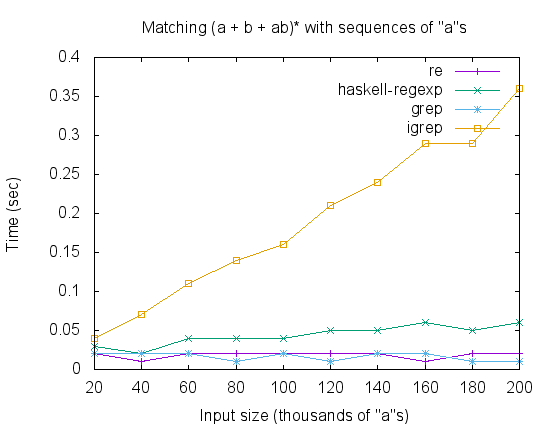
\includegraphics[width=0.7\textwidth]{as.png}
   \centering
   \caption{Results of experiment 1.}
   \label{fig:graph1}
\end{figure}

\begin{figure}[!ht]
    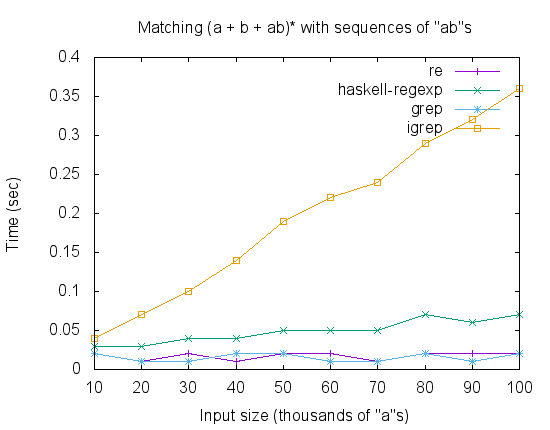
\includegraphics[width=0.7\textwidth]{abs.png}
   \centering
   \caption{Results of experiment 2.}
   \label{fig:graph2}
\end{figure}

Our tool behaves poorly when compared with all other options
considered. Possible causes for this inefficiency: 1) We represent
alphabet symbols as natural numbers in Peano notation which has
a costly equality test (linear on the term size); 2) our algorithm
relies on the Brzozowski definition of RE
parsing, which needs to quotient resulting REs. We believe that the
use of disambiguation strategies like greedy parsing~\cite{FrischC04}
and POSIX~\cite{SulzmannL14} would be able to improve the efficiency
of our algorithm without sacrificing its correctness. The usage of
these strategies can avoid the use of smart constructor to quotient
equivalent REs. We leave the formalization of such disambiguation
strategies for future work.

\section{Related Work}\label{sec:related}

\paragraph{Parsing with derivatives}: Recently, derivative-based parsing has
received a lot of attention. Owens et. al. were the first to present a
functional encoding of RE derivatives and use it to parsing and DFA
building. They use derivatives to build scanner generators for ML and 
Scheme~\cite{Owens2009} and no formal proof of correctness were
presented.

Might et. al.~\cite{Might2011} reports on
the use of derivatives for parsing not only RLs but also context-free
ones. He uses derivatives to handle context-free grammars (CFG) and
develops an equational theory for compaction that allows for efficient
CFG parsing using derivatives. Implementation of derivatives for CFGs
are described by using the Racket programming
language~\cite{Felleisen2013}. However, Might et. al. doesn't present
formal proofs related to the use of derivatives for CFGs.

Fischer et. al. describes an algorithm for RE-based parsing based on
weighted automata in Haskell~\cite{Fischer2010}.  The paper describes
the design evolution of such algorithm as a dialog between three
persons. Their implementation has a competitive performance when
compared with Google's RE library~\cite{re2}. This work also does not
consider formal proofs of RE parsing.

An algorithm for POSIX RE parsing is described
in~\cite{SulzmannL14}. The main idea of the article is to adapt
derivative parsing to construct parse trees incrementally to solve
both matching and submatching for REs. In order to improve the
efficiency of the proposed algorithm, Sulzmann et. al. use a bit
encoded representation of RE parse trees. Textual proofs of
correctness of the proposed algorithm are presented in an appendix.

\paragraph{Certified parsing algorithms}: Certified algorithms for
parsing also received attention recently. Firsov et. al.~describe a
certified algorithm for RE parsing by converting an input RE to an
equivalent non-deterministic finite automata (NFA) represented as a
boolean matrix~\cite{FirsovU13}. A matrix library based on some
``block'' operations~\cite{MacedoO13} is developed and used Agda
formalization of NFA-based parsing in Agda~\cite{Norell2009}. Compared
to our work, a NFA-based formalization requires a lot more
infrastructure (such as a Matrix library). No experiments with the
certified algorithm were reported.

Firsov describes an Agda formalization of a parsing algorithm that
deals with any CFG (CYK algorithm)~\cite{Firsov2014}. Bernardy
et. al.~describe a formalization of another CFG parsing algorithm in
Agda~\cite{BernardyJ16}: Valiant's algorithm~\cite{Valiant1975}, that
reduces CFG parsing to boolean matrix multiplication. In both works,
no experiment with formalized parsing algorithms were reported.

A certified LR(1) CFG validator is described
in~\cite{Jourdan2012}. The formalized checking producedure 
verifies if CFG and a automaton match. They proved soundness and
completeness of the validator in Coq proof
assistant~\cite{Bertot2010}. Termination of LR(1) automaton
interpreter is ensured by imposing a natural number bound.

Formalization of a parser combinator library was the subject of
Danielsson's work~\cite{Danielsson2010}. He built a library of parser
combinators using coinduction and provide correctness proofs of such
combinators.

\section{Conclusion}\label{sec:conclusion}

We have given a complete formalization of a derivative-based parsing
for REs in Idris. To the best of our knowledge, this is the first work
that presents a complete certification and that uses the certified
program to build a tool for RE-based search.

The developed formalization has 563 lines of code, organized in seven
modules. We have proven 23 theorems and lemmas to complete the
development. Most of them are immediate pattern matching functions
over inductive datatypes and were omitted from this text for brevity.

As future work, we intend to work on the development of a certified
program of greedy and POSIX RE parsing using Brzozowski
derivatives~\cite{SulzmannL14,FrischC04} and investigate about how
ways to obtain a formalized but simple and efficient RE parsing tool.

\paragraph{Acknowledgements:} The first author thanks Fundação de Amparo a
Pesquisa de Minas Gerais (FAPEMIG) for financial support.

\bibliographystyle{plain}
\bibliography{main}

\end{document}
